
\documentclass{article}
\usepackage[a4paper, top=1cm, right=2cm, bottom=1cm, left=2cm]{geometry}
\usepackage[onehalfspacing]{setspace}

\usepackage[utf8]{inputenc}
\usepackage[T1]{fontenc}
\usepackage{amsmath}
\usepackage{xargs}
\usepackage{tikz}


\title{\vspace{-2em}\Huge{\textbf{Chap 6 : Graphes}}\vspace{-1.5em}}
\author{}
\date{}

%\tgrph{ordre}[taille][rota(senstrigo)]
\newcommandx{\tgrph}[3][2=2, 3=0]{
\begin{tikzpicture}[transform shape]
    \foreach \x in {1,...,#1}{
        \pgfmathparse{\x*(360/#1)-(360/#1)+90+#3}
        \node[draw,circle,minimum size=0.5cm] (N-\x) at (\pgfmathresult:#2cm) {\x};
    }
    \foreach \x [count=\xi from 1] in {2,...,#1}{
        \foreach \y in {\x,...,#1}{
            \draw (N-\xi) -- (N-\y);
        }
    }
\end{tikzpicture}
}

%\ct{contents}[columns]
\newcommandx{\ct}[2][2=ccc]{
    \begin{center}
        \begin{tabular}{#2}
            #1
        \end{tabular}
    \end{center}
}

\begin{document}
    \maketitle
    \setlength{\parindent}{0cm}
    \bgroup\obeylines

    \section{Introduction aux graphes}
        \subsection{Vocabulaire}
            \subsubsection{Graphe non-orienté}
                Définition:
                \framebox[\linewidth][l]{Un graphe non-orienté G est un ensemble de sommets reliés par des arêtes.}
                Exemple:
                \ct{
                    Sommet & Arête & Graphe G\\
                    \tikz\node[draw,circle](1){1}; & \tikz\draw(0,0)--(1,0); & \tgrph{2}[0.5][90]
                }


        \subsection{Graphes complets}
            Définition:
            \framebox[\linewidth][l]{Un graphe non-orienté est dit complet si tous ses sommets sont adjacents.}
            Exemple:
            \ct{
                Ordre 5 & Ordre 7 & Ordre 9\\
                \tgrph{5} & \tgrph{7} & \tgrph{9}
            }


        \subsection{Graphes non-orientés et chaînes}
            \subsubsection{Chaînes}
            \subsubsection{Chaîne d'Euler}


    \section{Graphes orientés et lien avec les matrices}
        \subsection{Graphes orientés}
        \subsection{Matrices}
            \subsubsection{Matrice d'adjacence}
            \subsubsection{Puissances de matrices}


    \section{Pour aller plus loin}
        \subsection{Chaîne de Markov}

        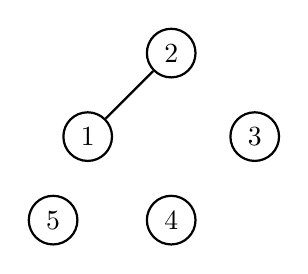
\begin{tikzpicture}[node distance={15mm}, thick, main/.style = {draw, circle}]
            \node[main] (1) {1};
            \node[main] (2) [above right of=1] {2};
            \node[main] (3) [below right of=2] {3};
            \node[main] (4) [below left of=3] {4};
            \node[main] (5) [left of=4]{5};
            \draw (1) -- (2);
        \end{tikzpicture}

    \egroup
\end{document}
